% this might be useful: \def\figpath{Figures/traversal/}

\chapter{Presenting Structured Documents}
\label{chap:presenting}

Xprez is not latex!! Latex is too complex. Xprez is target. Latex needs attributes and lot of computations. Proxima can build an editor for latex, but not just using Xprez. IE. fontsize etc will be visible in document level.

Cassowary is not cited in article


%---------- generated part:

The popularity of the document standard XML has led to an increasing demand for XML editors. The Proxima project is concerned with the design of a generic presentation-oriented XML editor with support for derived values in documents. A presentation is a view on a document, according to a style sheet. In a presentation oriented editor the user only sees a presentation of a document. WYSIWYG editing is possible using a WYSIWYG presentation, whereas the underlying document structure can be viewed and edited with a presentation that shows the actual tags and tree structure of the document. Because Proxima will support derived values, constructs such as chapter numbers and references are not hard-coded in the editor, but can be specified entirely by the user. Also, computations in a document, where one field contains the result of a calculation over several input fields can be modeled with derived values. In order to specify document presentations, a powerful presentation language is required. For this reason, we have developed the declarative XML presentation language {\sc Xprez}.

There exist a number of style sheet or presentation languages for XML, for example CSS~\cite{css}, CCSS~\cite{ccss}, PSL~\cite{psl}, XSL~\cite{xsl}, and P~\cite{thot}, but they lack either the expressiveness or the abstraction mechanisms to specify the complex presentations required for an XML editor. Pretty-printing combinators \cite{oppen,swierstra,hughes,kahl,brand} do offer expressiveness, abstraction mechanisms and first-class presentations, but most of these libraries only have combinators for text, and all of them require a program for traversing the document tree and generating the presentation. 

In a comparative study of a number of existing languages, we determined the following list of requirements for a presentation language:

\begin{itemize}
\item Complicated presentations should be possible, but at the same time simple presentations should be easy to specify.
\item The language should be declarative. Thus the order in which presentations are specified is not important.
\item Domain-specific syntax should be available for presentation specific constructs. 
\item It should support a flow (\`a la XSL) and a box (\`a la \TeX~\cite{tex}) model with alignment.
\item Presentations should be first-class values. Thus presentations can be manipulated, passed as arguments to functions, etc.
\item It should have a powerful abstraction mechanism. Thus similar presentations can be specified with one, appropriately parameterized, function.
\end{itemize}

{\sc Xprez} has been implemented in the functional language Haskell. It does not yet have a domain-specific syntax, but other than that it meets the requirements. Although the language is not yet fully developed, it is already powerful enough to describe a \LaTeX -like presentation with a style sheet of about 300 lines. Below are two screenshots of an example document presented using this style sheet. The style sheet handles section numbering, ligatures (e.g. the ``fi'' in Scientific), and several mathematical constructs.

\begin{center}
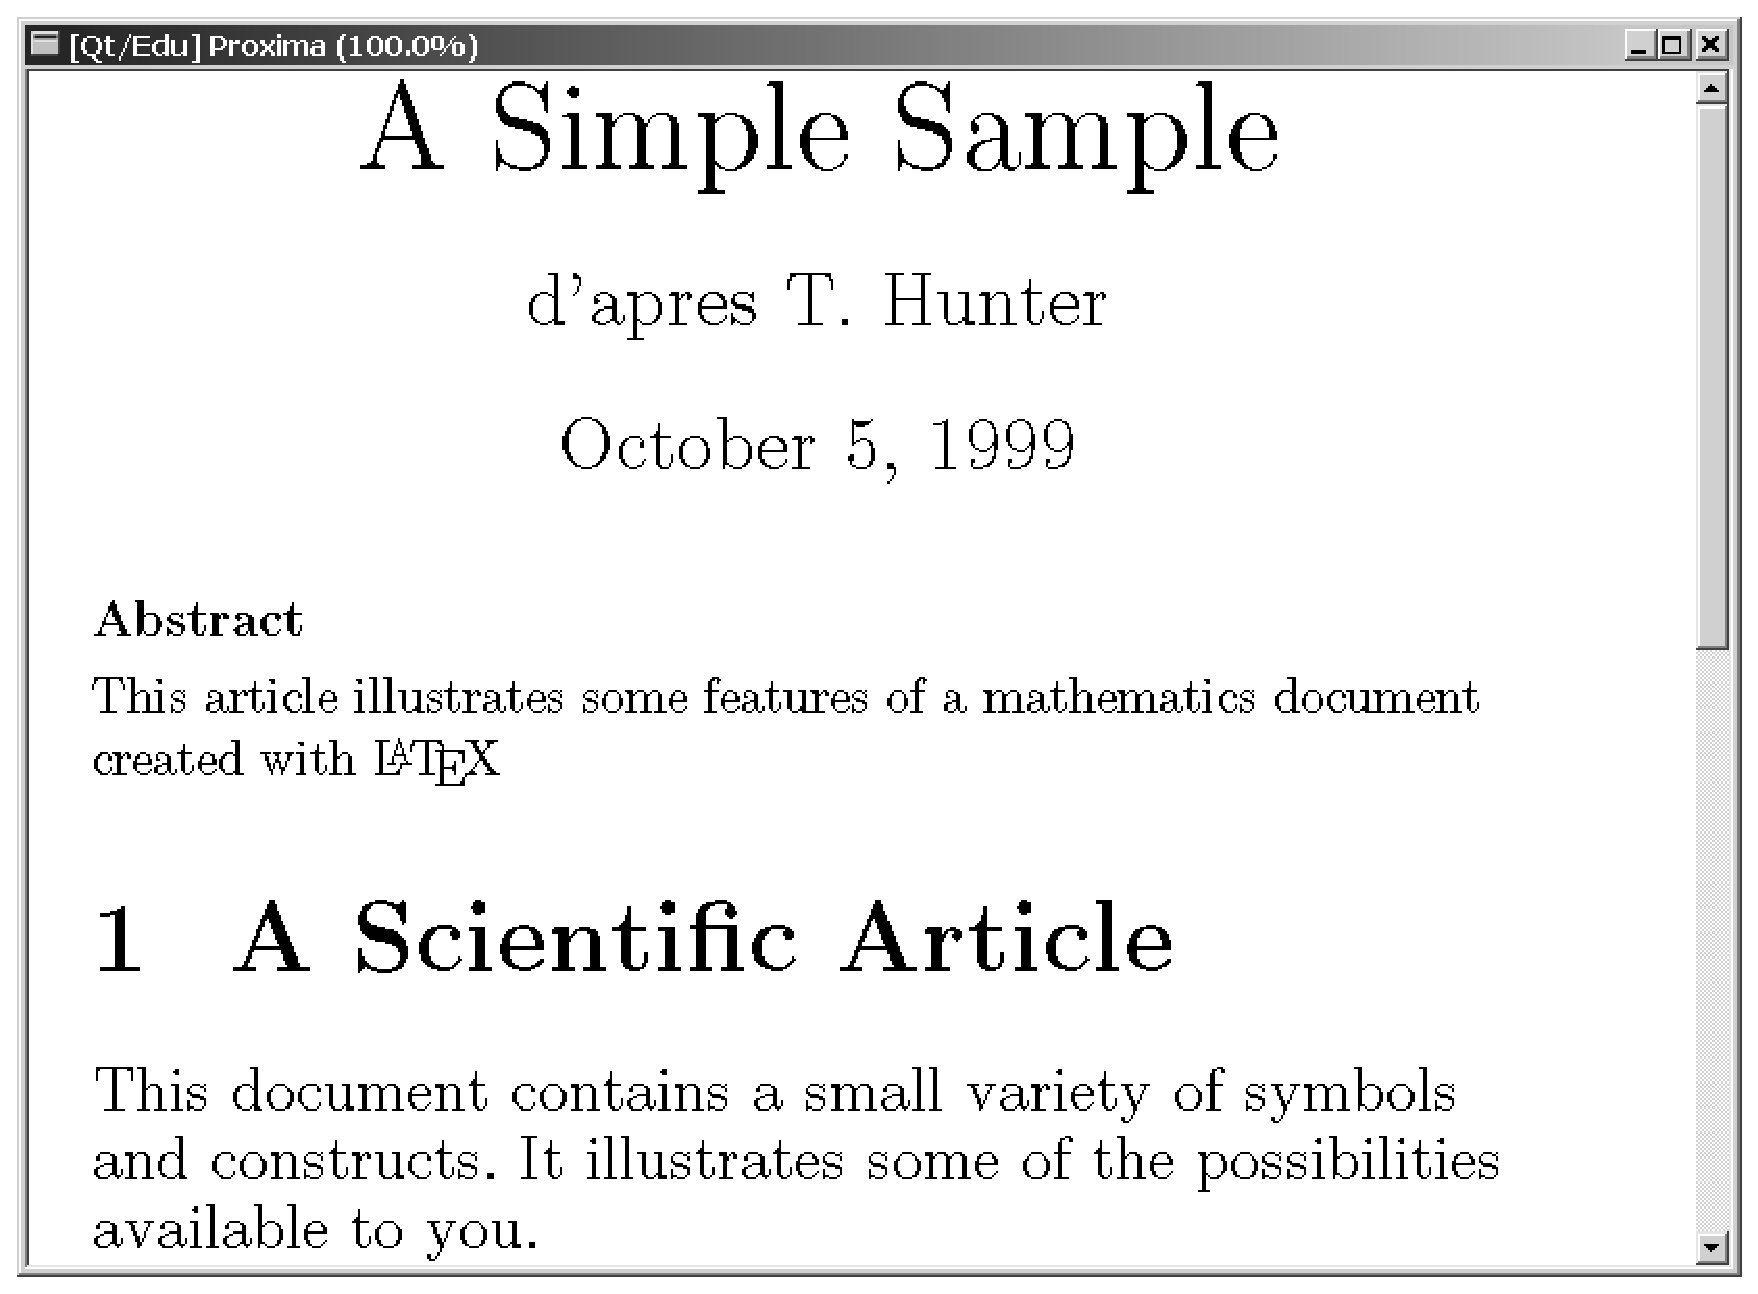
\epsfig{file=xprezpics/eps/xlatex1.png.eps, width=2in} \qquad
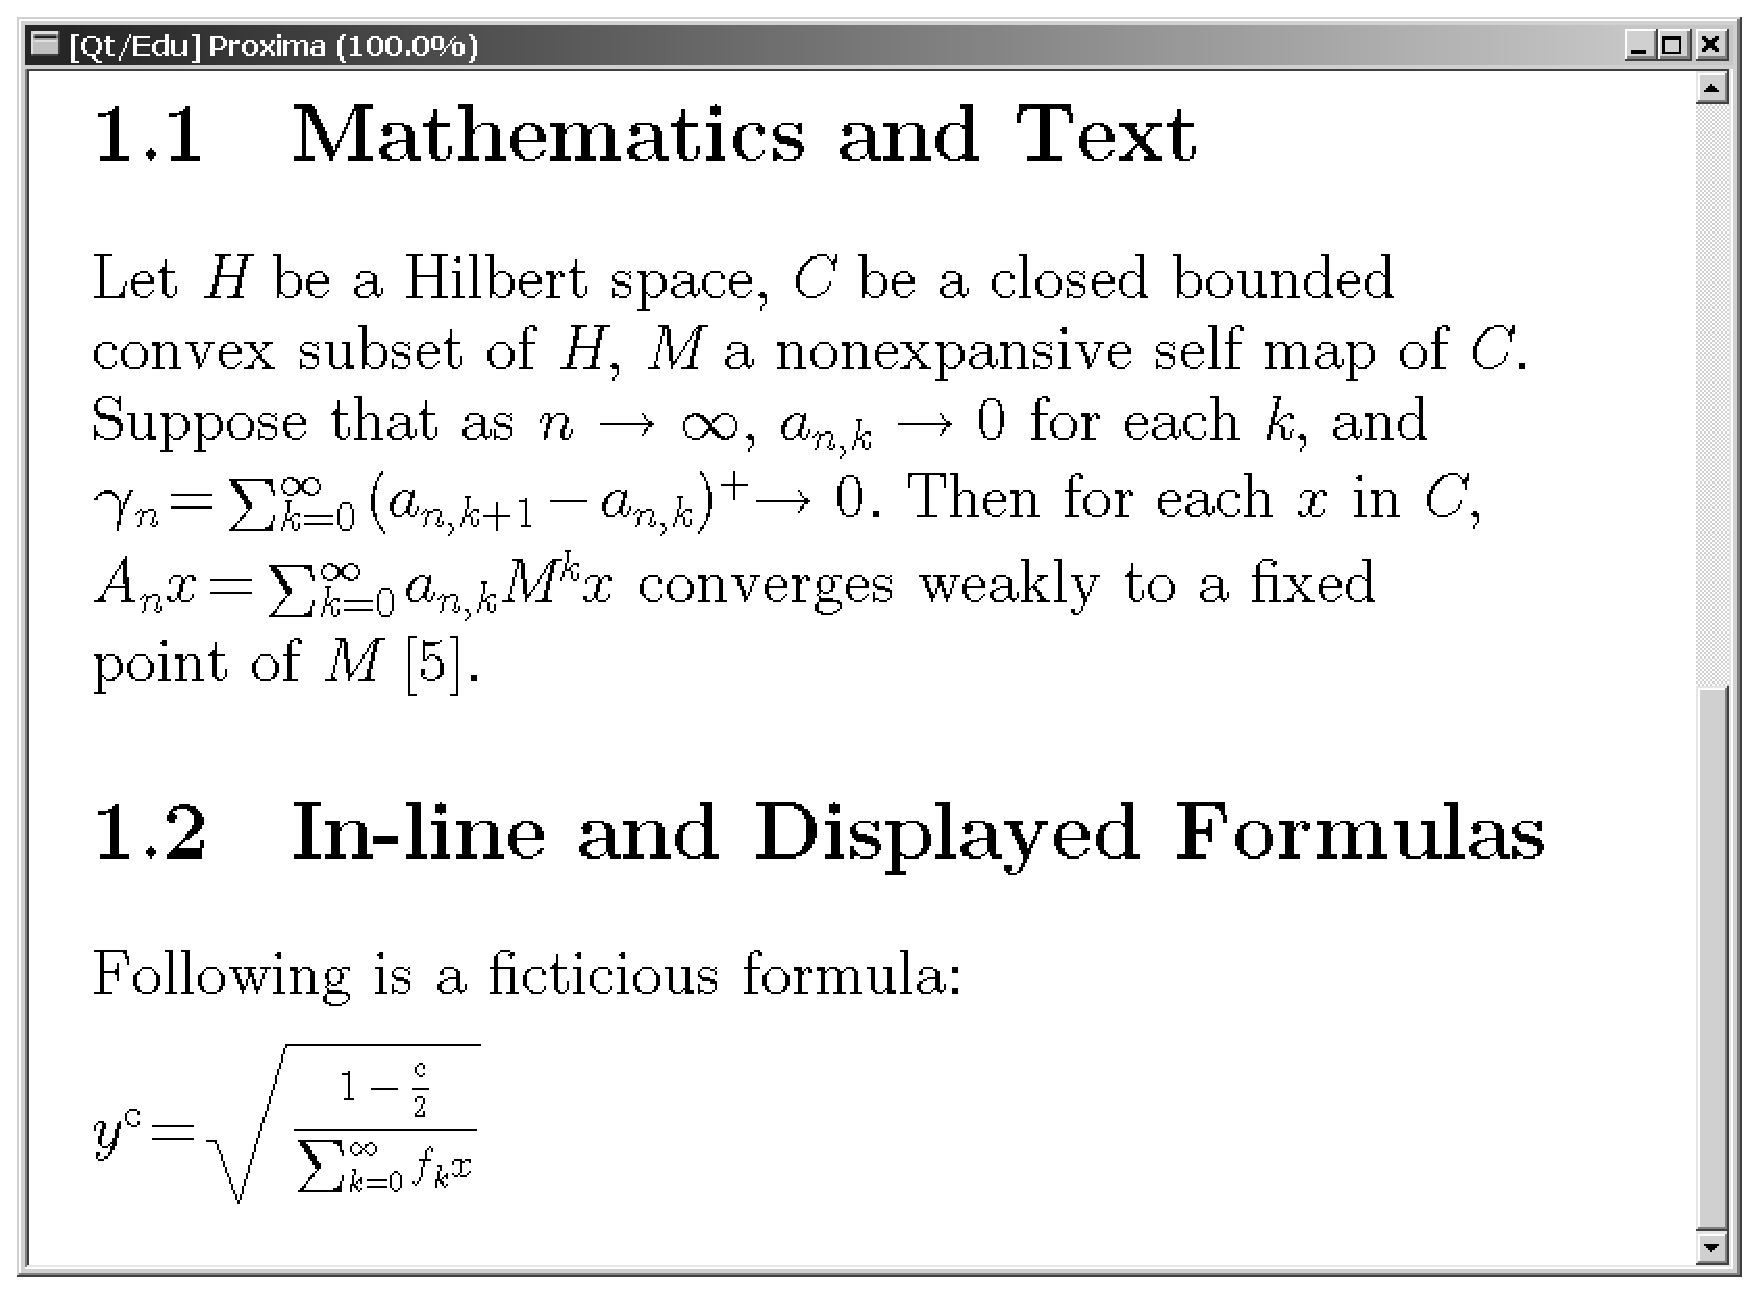
\epsfig{file=xprezpics/eps/xlatex2.png.eps, width=2in}
\end{center}

%Contributions of this paper:
The contributions of this paper are:

\begin{itemize}
\item An evaluation of the strengths and weaknesses of existing presentation languages, resulting in a list of requirements for a presentation language.
\item A proposal for the declarative presentation language {\sc Xprez} that supports both the flow and the box model, has presentations as first-class objects, and has a powerful abstraction mechanism.
\end{itemize}

%Paper organisation
Two kinds of languages are involved in the presentation process: a presentation target language, and a presentation specification or transformation language. The presentation target language describes the building blocks of the presentation that is shown on the screen or sent to a printer, whereas the transformation language describes how an XML document is mapped onto the target language to create this presentation. The Extensible Stylesheet Language (XSL) gives a clear example of the distinction, as it has been split into a transformation language (XSL Transformations or XSLT) and a target language (XSL Formatting Objects). XSLT documents specify transformations that map a source document tree to a tree of Formatting Objects, which can then be rendered. 

Section~\ref{targetlangs} discusses existing presentation target languages, followed by the introduction of the target language of {\sc Xprez} in Sect.~\ref{xpreztarget}. Section~\ref{transformlangs} deals with the transformation languages and Sect.~\ref{conclusions} concludes.


%									
%									
%									
\section{Presentation Target Languages}
\label{targetlangs}

The elementary building blocks of most presentation target languages are basic presentations of strings and small graphical objects such as lines, squares and circles. They can be composed according to a number of models:

\begin{description}
\item[Flow model]
When a flow model is used, presentations are placed next to each other or above each other, depending on the current flow direction. If the remaining space in the current direction is too small to fit the presentation, a new flow presentation is started. In this way, lists of words can be divided into lines and lists of lines can be divided into pages. The generated list of flows may then be manipulated further, for example, by extending each page in a list of pages with a header and a footer.
\item[Box model]
The box model allows each presentation to define its position relative to sibling or parent presentations. The positions can be set either directly by specifying them relative to positions of other presentations, or by declaring constraints. If constraints are used, the style sheet does not so much specify the exact calculation of a property, but rather gives constraints that should hold for the property. The actual computation of the property value is left to a constraint solver. 
\item[Matrix model]
The matrix model can be used to align a tree of cells, usually a list of rows that each contain a list of cells, along the rows as well as the columns. This is difficult to specify just using rules for each row and cell, as the width of the n-th cell has to be related to the n-th cells in the other rows instead of to properties of its parent or sibling cells. Matrices can be used to create box presentations, but the extent to which this is possible depends on the expressivity of the matrix model; for example, whether or not cells may overlap.
\item[Absolute positioning]
A very low level way of formatting is specifying the absolute coordinates in the resulting presentation.
\end{description}


%									
\subsection{Existing Presentation Target Languages} \label{existingtarget}

In this section, we will examine the target sublanguages of five presentation languages: CSS~2.0, CCSS, XSL, PSL and P. Of these five languages, only XSL regards its target language as a separate language with its own syntax. The other languages only describe how properties of the elements of the target presentation tree can be set, but they do not treat presentations as actual values in the language.

\bigskip{\bf CSS~2.0:} Cascading Style Sheets, level~2~\cite{css} is an example of a simple presentation language. Its target language is almost invisible to the style sheet designer. The presentation of a document is a tree that is almost isomorphic to document tree, with the document content in the leaves. It is not entirely isomorphic, because content can be left out and simple text content can be added. The nodes of the tree specify presentation properties such as font size or color, either absolutely or as a percentage, but arbitrary expressions are not allowed. The kind of a property determines to what property a percentage refers. For instance, a percentage value for the {\em font-size} property refers to the font size of the parent element, but a percentage for the {\em line-height} property refers to the font size of the element itself. It is not possible to let a property value depend on arbitrary properties of the parent or siblings in the presentation tree. CSS~2.0 supports a flow layout and absolute positioning. There is also a table format, but it is of limited use because the transformation language is rather weak. Consequently, if the data in the document does not have exactly the same structure as a CSS~2.0 table, it cannot be presented as one.

\bigskip{\bf CCSS:} Constraint Cascading Style Sheets~\cite{ccss} is an extension of the CSS~2.0 standard that is based on constraints. CCSS's target language closely resembles the CSS~2.0 target language, but child properties are specified using constraints instead of percentages of the parent's property values. Another difference is that the constraints can refer to global constraint variables and to left-siblings in the presentation tree as well as to the parent node. 

\bigskip{\bf XSL FO:} On the other side of the spectrum is the XSL language. The target language, XSL Formatting Objects, consists of a large collection of elements that can be used to specify page models, presentation properties, and more complicated presentation aspects, such as hyphenation and counters. A presentation is a tree that consists of these formatting objects. The style sheet offers strong control over the flow model, but no box model is supported. There is a table model, but using it to do a box layout is difficult, because the style sheet would then have to take care of the alignment, and XSLT does not support a strong computational formalism.

\bigskip{\bf PSL:} The Proteus Stylesheet Language~\cite{psl} is an attempt to combine the simplicity of CSS~2.0 with the power of XSL. Its target language is again close to the CSS target language. PSL extends the CSS target language with a box model and graphical symbols. The value of a property can be expressed as a mathematical expression that refers to properties of nodes in the presentation tree. This mechanism is called {\em property propagation}. PSL supports a constraint based box model. Presentations can specify their position and size properties relative to other presentations in the tree, which are addressed using a number of primitive functions for accessing siblings, parents and ancestors of a specified type, etc.

\bigskip{\bf P:} The last language considered here is the presentation language P of the Thot editor toolkit~\cite{thot}. It has a target language that consists entirely of boxes. Instead of having a large number of different presentation boxes, like the XSL Formatting Objects, P has only three kinds of boxes with a large number of properties. In contrast to PSL, the box layout in P is not constraint based, so the style sheet designer needs to take the order of computation of the layout properties into account. P does support horizontal and vertical reference lines for automatic alignment of boxes. Matrices are not primitive objects in P.

\bigskip{\bf Discussion:} The languages discussed above are all declarative and domain-specific languages that vary in expressive power. The simple languages CSS~2.0, CCSS, and PSL allow simple presentations to be specified in a simple way, but cannot be used to specify more complex presentations, such as mathematical formulas. In contrast, XSL and P do allow complex presentations to be specified, but due to the lack of abstraction, simple presentations also have rather elaborate specifications, especially in P. 

Only P and PSL support a box model, but both models are of a rather object-oriented and imperative nature. A box can specify its own position properties relative to its parent or siblings, but it is not possible to state at parent level that two child presentations should have their top and bottom aligned, or that two presentations should have the same width. As a consequence, a conceptually simple change of presenting the children of a node next to each other instead of above each other, requires changing the presentations for all child elements. Moreover, if the choice for vertical or horizontal layout depends on an attribute of the parent, then all children require code in their presentation rules for accessing this parent attribute, if possible, and letting their presentation depend on its value. If, however, presentations are first-class objects in the target language, then the parent presentation rule can specify the layout of the children.

Letting a child presentation specify its own layout makes it more difficult to understand a presentation. For example, a reverse order presentation of a list of children is obtained by aligning each right side with the previous child's left side. If, on the other hand, child presentations are first-class, and abstraction mechanisms can be used to define combinators on them, reversing can be specified by a simple reverse combinator. Another advantage of this approach is that the concepts of reversing and direction of layout are orthogonal now. Changing the layout from a horizontal list to a vertical list can be achieved by applying a different combinator to the reversed children, while the order of the children is controlled by applying the reverse combinator or not. In the P and PSL model, these concepts are intertwined.

\bigskip{\bf  Requirements:} Based on the previous discussion, we can conclude that a presentation target language, and in particular the target language for Proxima, will have to meet the following requirements: 

\begin{description}
\item[Proportional effort]
It must be possible to specify complex presentations, but the specification of simple presentations should still be easy.
\item[Declarative]
In a declarative language, understanding a composite presentation is easier, because the computation of a presentation does not generate side effects. Another advantage is that the designer does not need to worry about the order of computation of presentations and properties.
\item[Domain-specific]
The language should have syntax for presentation specific constructs such as an {\bf em} (height of the letter m in the current font and size) and different measuring units such as pixels and inches.
\item[Flow and Box model with alignment]
The language requires a flow model for textual parts of a presentation, and a box model for displaying mathematical formulas and other more graphical presentations such as trees. Automatic alignment is required in order to be able to specify composite presentations without having to explicitly position each child presentation.
\item[First-class presentations]
A first-class presentation can be named and manipulated at the level of its parent, which in many cases is the natural place to manipulate it. At the same time, it is still possible to specify properties at child presentation level, when this is more appropriate.
\item[Powerful abstraction mechanism]
User-defined functions and var\-i\-ables help to reduce code duplication, facilitate code reuse, and increase transparency, because complicated pieces of code may be replaced by functions with well-chosen names.
\end{description}


%									
%									
%									
\section{The {\sc Xprez} Target Language}
\label{xpreztarget}

With the requirements from the previous subsection in mind, we have developed the declarative presentation language {\sc Xprez}. 


%									
\subsection{{\sc Xprez} Presentation Model}

{\sc Xprez} is a box language, like P, and the document formatting languages \TeX ~and Lout~\cite{lout}. A presentation is a value of the abstract data type \texttt{Xprez}, the definition of which is omitted. A presentation is either a simple box containing a piece of text or a graphical object, or a composite box that contains a list of child presentation boxes. It can therefore be viewed as a tree in which the leaves are simple presentations and the nodes are composite presentations. We construct \texttt{Xprez} values in the functional language Haskell extended with a number of primitive functions that will be described in Sect.~\ref{primitives}.

\begin{figure}
\begin{small}
\begin{center}
\begin{small}
\begin{verbatim}
data Inh = Inh {fontFamily :: String, fontSize :: Int,
                textColor, lineColor, fillColor, backgroundColor :: Color} 
data Syn = Syn {hRef, vRef, minWidth, minHeight :: Int,
                hStretch, vStretch :: Bool}
\end{verbatim}
\end{small}
\caption{The {\sc Xprez} properties}\label{xprezproperties} 
\end{center}
\end{small}
\end{figure}
\pagebreak

A presentation box (from now on called presentation) has a number of properties that describe its size and its appearance: 

\begin{center}
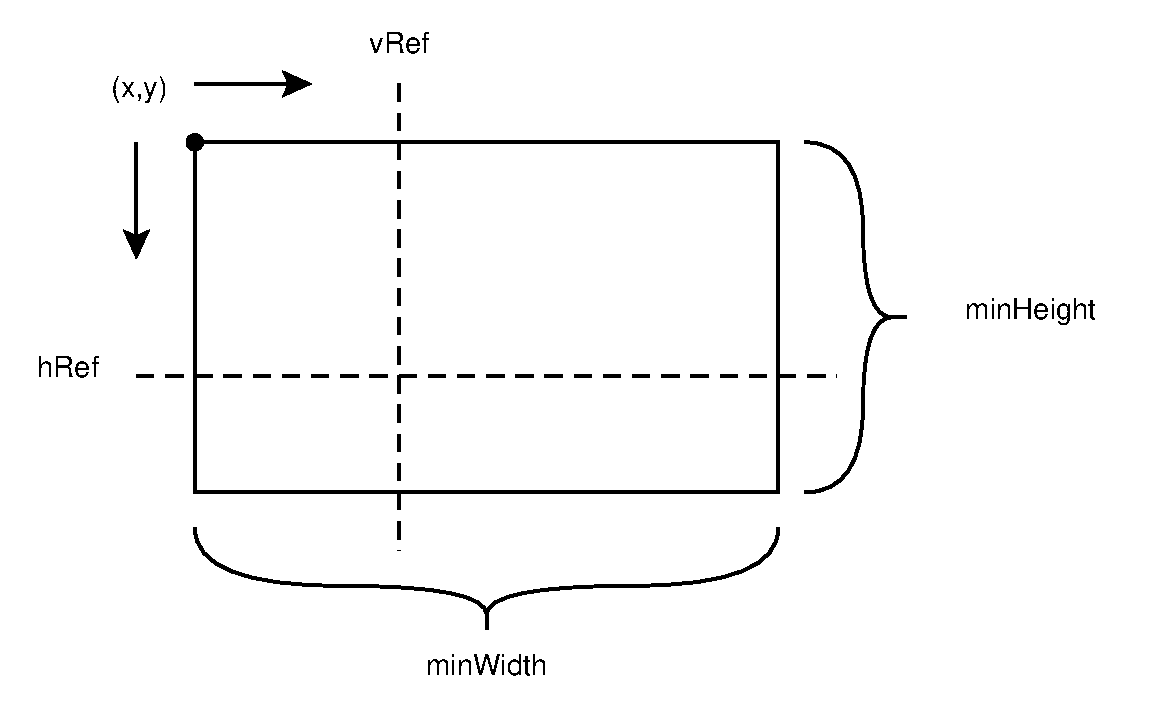
\epsfig{file=xprezpics/eps/picob.eps, width=2in}
\end{center}

\noindent Figure~\ref{xprezproperties} contains the definition of the two records \texttt{Inh} and \texttt{Syn} (as explained below) with the type of each of the properties. The \texttt{hRef} and \texttt{vRef} properties specify the horizontal and vertical reference lines that are used for aligning boxes when they are combined in composite presentations. The boolean properties \texttt{hStretch} and \texttt{vStretch} specify whether or not the presentation is allowed to stretch in horizontal or vertical direction. The rest of the properties are \texttt{fontFamily}, \texttt{fontSize}, \texttt{textColor}, \texttt{lineColor}, \texttt{fillColor}, and \texttt{backgroundColor}, which should be self explanitory. In the future, this set will be extended with other properties such as more line style and font attributes, and user defined properties will be supported. The presentation tree is transformed into an attribute grammar in which the font, style, and color properties are inherited attributes that go down in the tree, and alignment and stretch properties are synthesized attributes that go up in the tree. In the Haskell types, this division is visible in the fact that the properties are modeled using two records: \texttt{Inh} for inherited properties, and \texttt{Syn} for synthesized properties.


%									
\subsection{{\sc Xprez} Primitives} \label{primitives}

Simple presentations can be created with the first five combinators in Fig.~\ref{xprezprim}. The \texttt{empty} combinator is a neutral element that is not visible and takes up no space. A piece of text can be presented with \texttt{text}, and a rectangle with \texttt{rect}, which takes the width and height as arguments. The \texttt{poly} combinator takes a list of relative coordinates between (0,0) and (1,1) and produces a line figure that connects these points. A \texttt{poly} presentation stretches in horizontal and vertical direction. Finally, \texttt{img} can be used to display bitmap images. The argument is a string that contains the path to the bitmap file. By default, the reference lines of simple presentations are 0, except for the horizontal reference line of a text presentation, which is equal to the baseline of the current font.

\begin{figure}
\begin{small}
\begin{center}
\begin{small}
\begin{verbatim}
empty             :: Xprez
text              :: String -> Xprez             -- simple text
rect              :: Int -> Int -> Xprez         -- rectangle
img               :: String -> Xprez             -- image (jpg, png, ...)
poly              :: [ (Float, Float) ] -> Xprez -- poly line
row, col, overlay :: [ Xprez ] -> Xprez          -- row, column, overlay
rowR, colR        :: Int -> [ Xprez ] -> Xprez   -- row, col w/ reference
matrix            :: [[ Xprez ]] -> Xprez
format            :: [ Xprez ] -> Xprez
\end{verbatim}
\end{small}
\caption{The {\sc Xprez} primitives}\label{xprezprim} 
\end{center}
\end{small}
\end{figure}

There are several kinds of composite presentations, the simplest being rows and columns (combinators \texttt{row} and \texttt{col}), which are duals. In a row, each child presentation is placed immediately to the right of its predecessor, with their horizontal reference lines aligned. Vertical reference lines have no effect on the positioning in a row.

\begin{center}
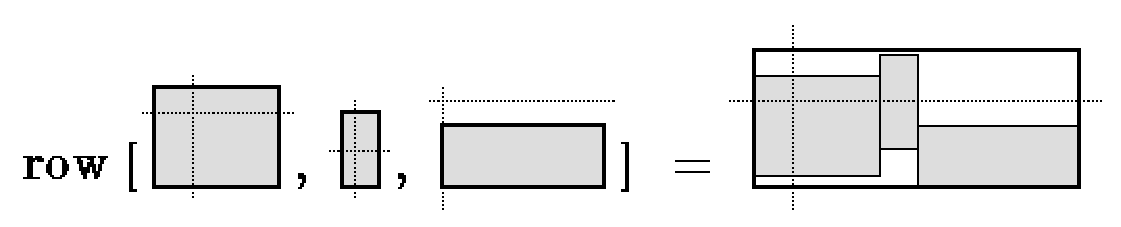
\epsfig{file=xprezpics/eps/row.png.eps, width=2.5in}
\end{center}

\noindent The bounding box of a row is the smallest rectangle that encloses all its children. The horizontal reference line is equal to the aligned reference lines of the children, whereas the vertical reference line is taken from one of the children (by default the first one). The \texttt{rowR} combinator takes an extra argument of type \texttt{Int} that specifies which child carries the vertical reference line for the row. \texttt{}By default, a row stretches in horizontal direction if one of its children does, and it stretches in vertical direction if all children stretch vertically. However, by setting the stretch properties, these defaults can be overridden. 

The \texttt{matrix} combinator can be used to describe a table layout, in which elements are aligned with elements to their left and right as well as with elements above and below them. 

Because \texttt{row}, \texttt{column} and \texttt{matrix} do not allow their children to overlap, a special combinator is required to create overlapping presentations. The \texttt{overlay} combinator places its children in front of each other, while aligning both the horizontal and vertical reference lines. It can be used to create underlined text, for example. Because alignment takes place on both reference lines and hence all child reference lines overlap, no special \texttt{overlayR} combinator is needed. 

The last composite combinator in Fig.~\ref{xprezprim} is \texttt{format}. It takes list of presentations as argument and splits this list into rows based on the available horizontal space. The resulting rows are placed in a column. The \texttt{format} combinator can be used to display a paragraph of words, or any other kind of presentations for that matter, on a number of lines. 

Here is an example {\sc Xprez} presentation that illustrates alignment and stretching in a row:

\begin{small}
\begin{verbatim}
let cross     = poly [(0,0),(1,0),(1,1),(0,1),(0,0),(1,1),(0,1),(1,0)]
    greycross = cross `withbgColor` grey
in  row [ text "Big" `withFontSize` 200
        , colR 2 [ cross, cross, text "small", greycross, greycross ] ] 
\end{verbatim}
\end{small}

\noindent This produces the following image (the dashed line has been added and represents the horizontal reference line of the presentation):

\begin{center}

\epsfig{file=xprezpics/eps/align.png.eps, width=1in}
\end{center}

The second element in the row is a column that takes the horizontal reference line from its third child (the numbering starts at 0), so the word {\bf ``Big''}, displayed with a font size of 200 pixels, is aligned with the word {\bf ``small''}, which has the default font size. The \texttt{cross} object is a line figure in the form of an X, and the \texttt{greycross} is that same figure with a grey background color. Because these presentations stretch in vertical direction, so does the column that contains them. The two stretching objects above the reference object (\texttt{text "small"}) are each assigned equal amounts of the remaining space above the horizontal reference line, and likewise, the objects underneath the reference object are assigned the remaining space below the reference line. If, on the other hand, the reference object itself is allowed to stretch, then the total amount of available space is added and distributed equally over all stretching objects. In this case, there will no longer be any alignment of the reference object. 


%									
\subsection{Property Modification}

The properties of a presentation can be modified using the generic \texttt{with\symbol{95}}\footnote{The name contains an underscore because Haskell already has a keyword {\em with}} combinator:

\begin{small}
\begin{verbatim}
with_ :: Xprez -> ((Inh, Syn) -> (Inh, Syn)) -> Xprez
\end{verbatim}
\end{small}

In the specification of a property value, the original values of properties can be used, e.g. the font size can be set to the old font size increased with 2 points. Therefore, the second argument of \texttt{with\symbol{95}} is a function that takes the original values of the inherited attributes that come from the parent and the synthesized attributes that come from child presentation as arguments, and returns the new values (i.e. the inherited attributes that go to the child and the synthesized attributes that go to the parent).

The inherited and synthesized property values are Haskell records, which have special syntax for accessing and updating fields. If \texttt{inh} is a value of type \texttt{Inh}, then the expression \texttt{fontSize inh} denotes the value of the fontSize field in \texttt{inh}, and \texttt{inh $\{$ fontSize = 10 $\}$} denotes a value of type \texttt{Inh} in which all fields have the same values as in \texttt{inh}, except for the \texttt{fontSize} field, which is now 10. Below is the definition for the \texttt{withFontSize} combinator: 

\begin{small}
\begin{verbatim}
withFontSize :: Xprez -> Int -> Xprez
withFontSize xp fs = xp `with_` \(inh, syn) -> (inh {fontSize = fs}, syn)
\end{verbatim}
\end{small}

Constructing functions comes with some syntactic overhead, but by using a libary of combinators for the most frequent uses, most of the calls to the actual \texttt{with\symbol{95}} combinator can be avoided. However, a problem with this derived combinator is that is that the \texttt{fs} value is of type \texttt{Int}, and therefore cannot depend on the original font size value. A different combinator that takes a function of type \texttt{Int -> Int} as argument, which is used in the fraction example below, solves this problem:

\begin{small}
\begin{verbatim}
withFontSize_ :: Xprez -> (Int -> Int) -> Xprez
withFontSize_ xp ffs = 
  xp `with_` \(inh, syn) -> (inh { fontSize = ffs (fontSize inh) }, syn)
\end{verbatim}
\end{small}

With \texttt{p `withFontSize\symbol{95}` (\symbol{92}fs -> 2*fs)} we can now specify the doubling of the font size for a presentation \texttt{p}, but again, this requires a function in the presentation code, although it is easier to write than the functions required by \texttt{with\symbol{95}}. A more natural solution is the declaration of a special data type \texttt{Length}, with operations such as addition and multiplication, but which also has primitive values that represent current font properties. In Haskell, type classes can be used to accomplish this. Using type classes, it will be possible to write: \linebreak \texttt{hSpace (2*em)}, which denotes a horizontal space of twice the height of the letter m in the current font. A future version of {\sc Xprez} will support special syntax for \texttt{with\symbol{95}}, so \texttt{text "a" with $\{$ child.fontSize = parent.fontSize * 2 $\}$} can be written without explicit functions.

The font size combinators show how abstraction is used to meet the {\em proportional effort} requirement. For simple changes of the font size, the simple \texttt{withFontSize} combinator can be used, and only if more control is desired, it is necessary to use the more complicated \texttt{withFontSize\symbol{95}} or \texttt{with\symbol{95}} combinators.


%									
\subsection{Advanced Examples}

A presentation in {\sc Xprez} is a first class value, so it is possible to perform manipulations on child presentations, such as positioning or font size updates, at parent level. This is illustrated in the following presentation for mathematical fractions: 

\begin{small}
\begin{verbatim}
frac e1 e2 = let numerator   = hAlignCenter (pad (shrink e1) )
                 bar         = hLine
                 denominator = hAlignCenter (pad (shrink e2) )
             in  colR 2 [ numerator, vSpace 2, bar
                        , vSpace 2, denominator ] `withHStretch` False

pad xp = row [ hSpace 2, xp, hSpace 2 ]

shrink e = e `withFontSize_` (\fs -> (70 `percent` fs) `max` 10)
\end{verbatim}
\end{small}

\noindent The non-primitive library function \texttt{hAlignCenter}, centers its argument horizontally, and the \texttt{shrink} function reduces the font size to 70\%, with a minimum of 10. The result of \texttt{(text "x" `frac` text "2") `frac` text "1 + y"} is:

\begin{center}
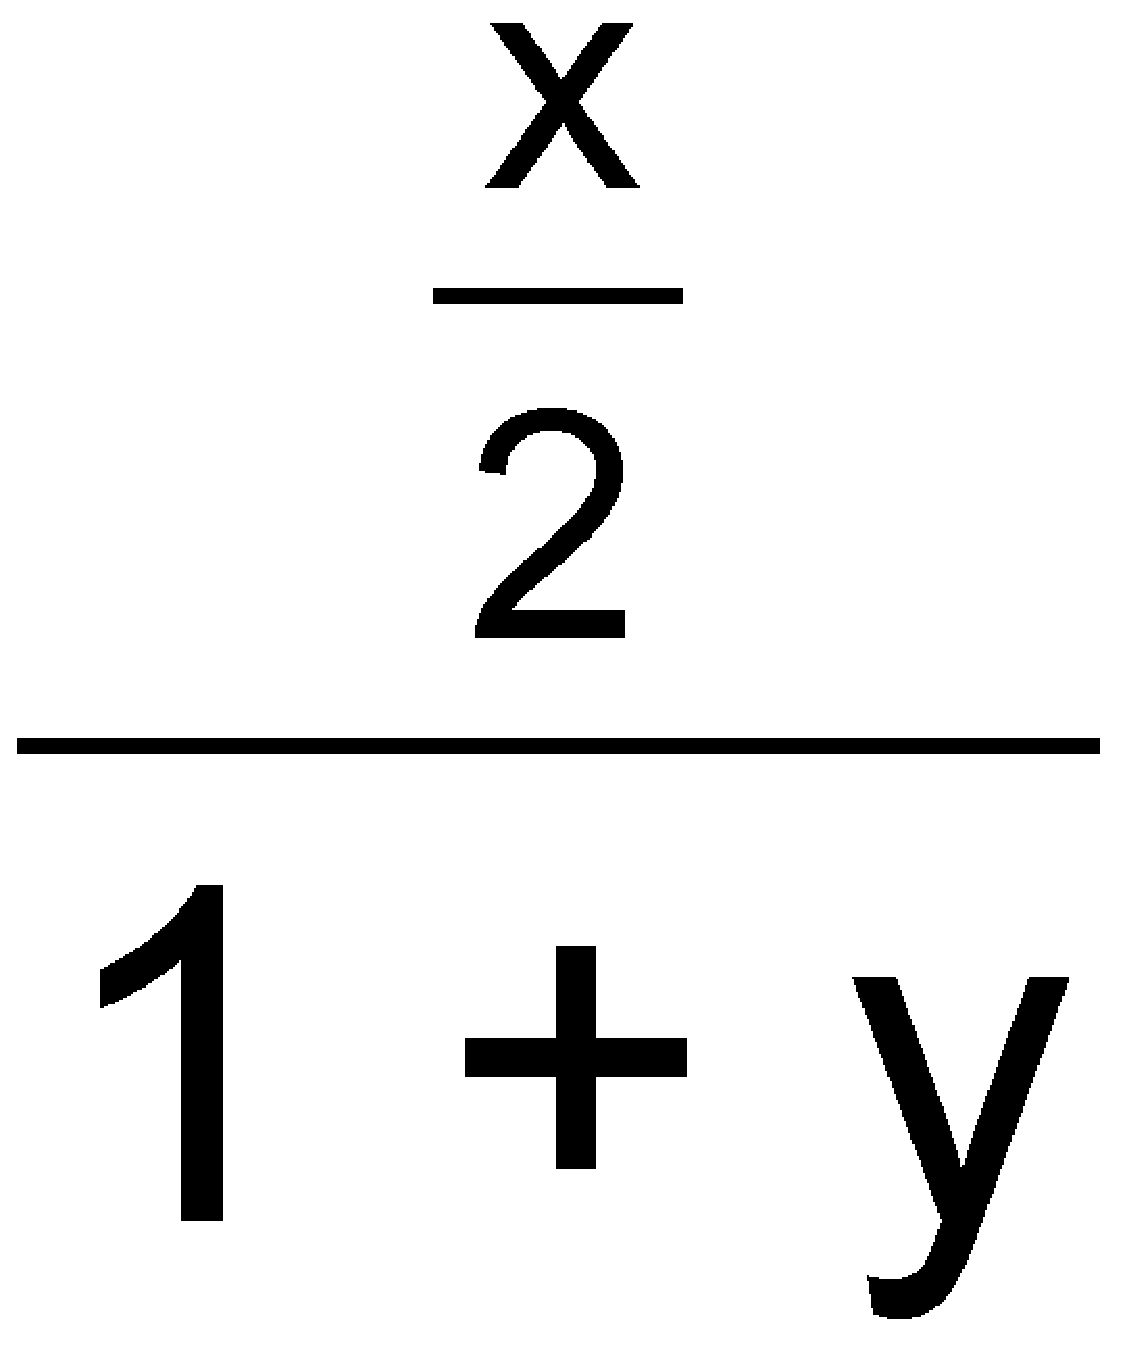
\epsfig{file=xprezpics/eps/frac.png.eps, width=0.5in}
\end{center}

The \texttt{pad} and \texttt{shrink} functions illustrate the {\em first-class} and {\em abstraction} requirements. Because a presentation is a first-class values, the presentations of the numerator and the denominator can be addressed and manipulated in the presentation of the fraction. Furthermore, using abstraction, the manipulations can be captured in the functions \texttt{pad} and \texttt{shrink}. In contrast, child presentations in both P or PSL cannot be addressed at parent level, so the fraction presentation must be created by letting each child, including the fraction bar specify its appearance and relative position. As a result, it is difficult to reuse parts of a presentation in another presentation, since all parts refer to each other, and the manipulations on the appearance are harder to read, because no abstraction can be used. 

The second example is a pair of combinators that can be used to create tree browser presentations:

\begin{center}
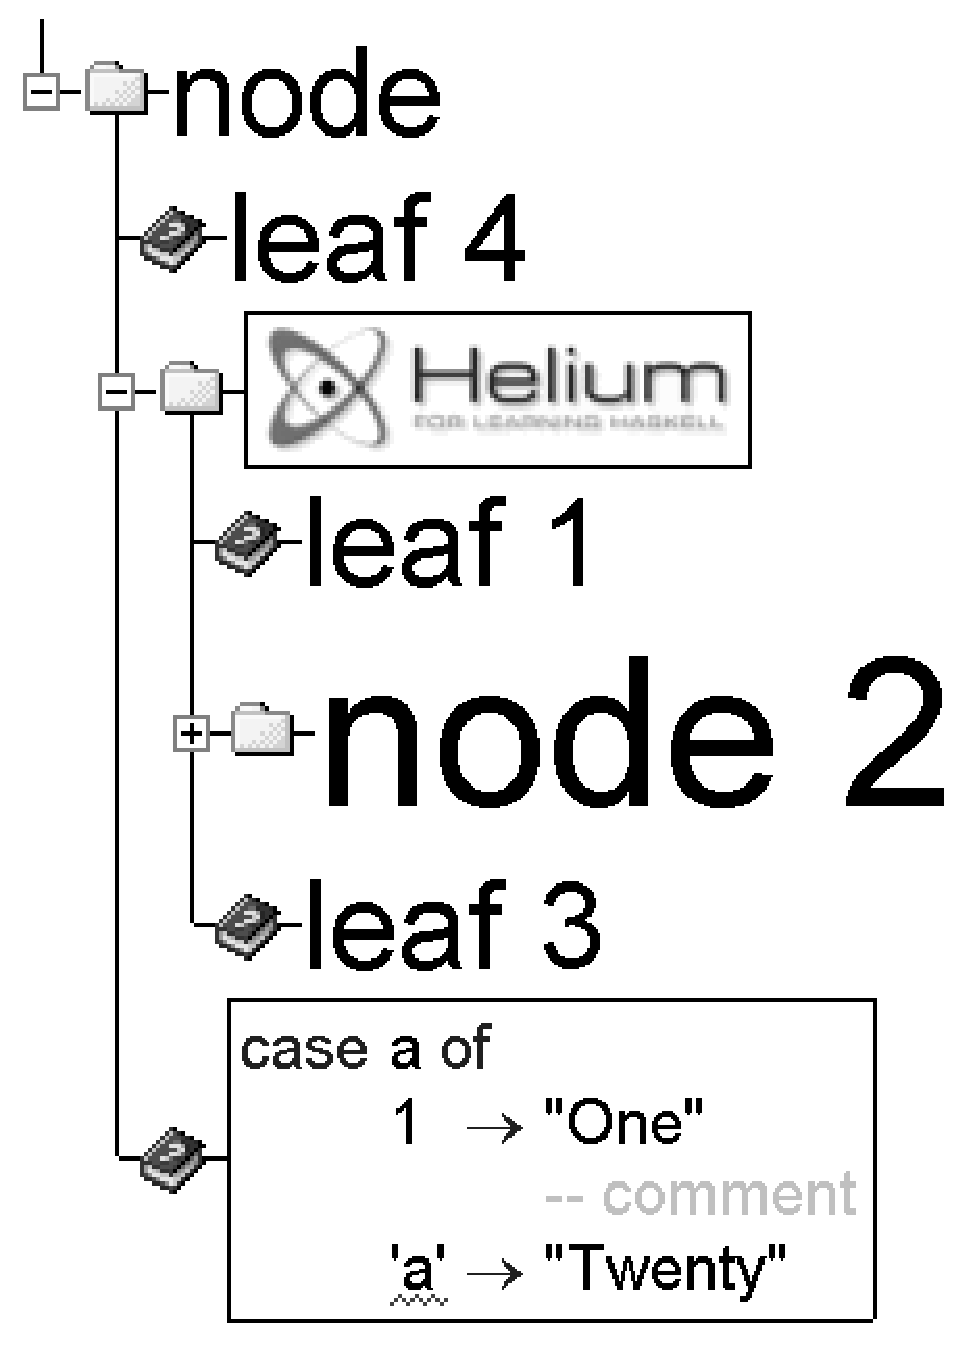
\epsfig{file=xprezpics/eps/tree.png.eps, width=1in}
\end{center}

\noindent This image has been created with the \texttt{mkTreeLeaf} and \texttt{mkTreeNode} combinators, which are defined in 20 lines of {\sc Xprez} code (see the Appendix for the source). Both combinators take an \texttt{Xprez} argument that is the presentation of the label, and the tree node also takes a list of child presentations (which should be either nodes or leaves for a correct tree, but can actually be any value of type \texttt{Xprez}). Labels are not restricted to text, but can also be images, or composite {\sc Xprez} presentations, like the label that contains the case expression in the last leaf of the example tree. 

The tree example is given here to show that a rather complex and graphical presentation can be specified with relatively little effort. However, in order to make this presentation a fully operational tree browser that can react to mouse clicks, we need to model the presentation state and edit operations on this state. This is not possible in the current version of {\sc Xprez} but will be possible in the Proxima editor system.


%									
\subsection{Future Work}

{\sc Xprez} meets the requirements listed at the bottom of Sect.~\ref{existingtarget}, with the exception of the domain-specific syntax, for which a special parser will have to be added to the system. Furthermore, there are a number of things that are still lacking in the current model and that are being investigated. Firstly, there is no page model yet, and hence no page related concepts such as footnotes and page references are possible. Probably, an abstraction similar to the {\em Galley} from Lout~\cite{lout} can be used for this. Secondly, there is no primitive notion of padding, which will allow spacing in columns and rows to be specified more naturally. Both of these concepts are related to the need for a more powerful \texttt{format} primitive that can handle both horizontal and vertical formatting while offering more control over the generated rows and columns. Finally, the \texttt{with\symbol{95}} combinator only gives access to the properties of a parent and its child. It is not possible to access properties of siblings, or presentations elsewhere in the tree, but it is also not yet clear whether such access is really necessary in a presentation language. Nevertheless, the set of combinators presented so far is powerful enough to cover much of the \TeX ~math typesetting as described in \cite{functionaltex}, including superscripts and subscripts. We also expect that defining a presentation sheet for the MathML~\cite{mathml} language will be rather straightforward in {\sc Xprez}.


%									
%									
%									
\section{Presentation Transformation Languages}
\label{transformlangs}

A presentation transformation language is used to specify a mapping between a document language (a subset of XML defined by a DTD) and a presentation target language. It may be a complete programming language, which is powerful, but leaves the burden of traversing the document structure on the programmer. Therefore, often a rule based language is used. For each element in the document type, one or more rules can be specified, which map the element onto its presentation. 


%									
\subsection{Existing Languages}

The five languages discussed in Section~\ref{targetlangs} all have rule-based transformation languages. However, the power of the rule selection mechanisms varies, as well as the transformation capabilities.{\bf }

{\bf CSS~2.0:} In CSS~2.0, rules are used to specify the appearance of elements or classes of elements. These rules are either applied to certain types of elements (e.g. all \texttt{Title} elements in the document), or depend on contextual information of an element (e.g. all elements that are a child of a \texttt{Section} element). The body of a rule consists just of property declarations.

It is possible to leave out the presentation of certain elements, and to add textual content before or after a presentation element in CSS~2.0, but general tree transformations cannot be specified. It is also not possible to specify computations. Therefore, a more complicated presentation structure, such as a table of contents or a section reference is impossible to specify using CSS~2.0. Frequently used derived values, such as element counters, have been added as primitives to the language, but they are not very flexible. Furthermore, the addition of special cases instead of a general solution, increases the complexity of the semantics of the language.

\bigskip{\bf CCSS:} The constraint mechanism of CCSS offers a more flexible rule selection. If the presentation environment differs from the one the designer had in mind, causing rules to fail, constraints can still specify an acceptable presentation, because they degrade continuously instead of discreetly. In CSS~2.0, a rule either succeeds or fails, but does not say anything about an approximate solution, leaving the choice to the rendering agent instead of to the style sheet designer. As a concrete example, it is possible to specify with constraints that no fonts should be smaller than 11 points, but if the actual font is at least 11 points, then this actual size should be chosen. Finally, CCSS also allows the specification of global constraints. For example all tables can be constrained to have the same width, without actually specifying this width.

\bigskip{\bf XSLT:} XSLT has a more powerful rule selection mechanism than the other languages discussed here. Specifying a rule to apply only to an element that is the second child of its parent, for example, is possible in XSLT but not in the other languages. XSLT supports conditional processing with if and case expressions based on document content or attribute values. However, the most important difference with the other languages is the fact that the resulting transformed tree need not be isomorphic to the document tree. The style sheet can direct the transformation process, supporting multiple passes over the document tree and allowing full structural transformations of the document. Unfortunately, XSLT does not allow the application of the style sheet to generated parts of the tree. This means that derived structures must be specified directly in the target language, whereas it would be more elegant to specify them in terms of the document language. In other words, it is not possible to specify derived document parts using logical markup instead of physical markup, as the former one would require another transformation pass over the generated tree. \note{Future: add an example}

\bigskip{\bf PSL:} The transformational capabilities of PSL are slightly weak\-er than those of XSLT, because the only way to influence the resulting tree is by extending the presentation tree with so called tree elaborations. Reversing a list of children is not possible in general, but can be simulated by having each child presentation put itself in front of the presentation of its predecessor. However, the resulting tree follows the structure of the original document tree, and a table of contents, for example, which requires a double pass over the document tree, cannot be specified elegantly in PSL.

\bigskip{\bf P:} In P, each element type has only one rule. An element presentation that depends on contextual information can be specified using conditionals that depend on the document structure. So instead of having a special rule for each possible parent an element may have, there is only one rule that alters its behavior based on the elements parent. A conditional presentation may also be based on a number of other factors, including document attributes and counter values, but no general boolean expressions are allowed. An important difference between P and the other presentation languages is that several views can be explicitly defined in the style sheet. 

\bigskip{\bf Discussion:} None of the discussed presentation languages have good support for abstraction. Only XSLT allows the definition of functions and variables, but these come at a high syntactic overhead, and no higher-order functions can be defined. As a result, a style sheet for a larger document type in which many elements have a similar presentation, becomes cluttered with a large number of rules that differ only in very few aspects. If all those rules were able to refer to one parameterized rule with as its parameters the variable aspects, then the style sheet would become more readable.

Another problem with these languages is that it is difficult to specify computations other than the basic counters that are provided as primitives. PSL allows computations on properties, but not on the content of the presentation. Specifying a field in the presentation that contains as its content the sum of a number of other fields is not possible. XSLT has very basic support for manipulations on numbers, text and booleans, but relies on separate scripting languages for more interesting calculations. However, the standard does not specify how a style sheet should be extended with scripting functions, and hence this is implemented differently by each XSLT processor. This makes it impossible to specify computations in a uniform and portable way.


%									
\subsection{{\sc Xprez} Transformation Language}

The transformation language for {\sc Xprez} is an attribute grammar over the document type. For each element, a synthesized attribute {\em pres} of type \texttt{Xprez} is defined, which specifies the presentation of the element. Apart from the presentation attribute, the style sheet designer can declare other synthesized and inherited attributes, in order to create derived document structures or perform computations over document values. Below is a presentation rule for the top-level \texttt{Module} element of a document type for a small functional language:

\begin{small}
\begin{verbatim}
Module name decls {
  pres = col [ row [ keyword "module ", name.pres, keyword " where" ]   
             , col decls.pres ] `withFont` ("Arial", 20)
}
\end{verbatim}
\end{small}

The attribute definitions are written in Haskell and can contain references to inherited attributes coming from the parent, as well as to synthesized attributes of the children, e.g. the presentations of the children. {\sc Xprez} has built-in support for XML lists and optional data types that takes care of propagating attributes through the document. If, for example, an element \texttt{E} has a synthesized attribute of type \texttt{a}, then a list of elements \texttt{E}, denoted in the DTD by \texttt{E*}, automatically has a synthesized attribute of type \texttt{[a]}. Because the attribute definitions are Haskell, abstraction can be used and regularly used patterns can be captured with functions. Moreover, computations over the document can make use of the full Haskell language.

As in P, only one presentation can be specified for each element. Context specific presentations have to be encoded using attributes. For example, by using an inherited attribute that contains the elements on the path to the root, an element can let its presentation depend on the type of its parent, or the presence of certain elements among its ancestors. Specifying such an attribute for each element in the document type is a hassle, so a collection of pre-defined attributes (e.g. positions, sibling lists, etc.) is present. 

The transformation component of {\sc Xprez} has been realized in Haskell, using the MAG attribute grammar system\cite{ag}. Currently, the system can handle only a subset of all document types, as there is no support for XML attributes and entities yet.


%									
%									
%									
\section{Conclusions}
\label{conclusions}

Current style sheet languages lack either the expressiveness or the abstraction mechanisms to specify complex presentations in a readable way. The declarative presentation language {\sc Xprez}, introduced in this paper, combines a flow and box model with a powerful abstraction mechanism and first-class presentations. The language is well suited for specifying a wide range of presentations, from tree browsers to WYSIWYG presentations of mathematical formulas, using concise and readable style sheets.

A Haskell implementation has been developed for both the target and transformation parts of {\sc Xprez}. It has been used to generate all screen shots in this paper. The user interface of this implementation is still in a premature stage, and the dependency on a number of different tools make it difficult to install. However, these are minor problems which require a fair amount of programming, but pose no major theoretical difficulties. For more information about the system, contact the authors, or visit: \url|http://www.cs.uu.nl/research/projects/proxima/|

\smallskip\noindent{\bf Acknowledgements:}

\noindent The authors thank Xander van Wiggen for implementing the Xprez renderer, and Dave Clarke and Doaitse Swierstra for their helpful comments on this paper.
